\documentclass{ximera}
\usepackage{sagetex}
%% handout
%% space
%% newpage
%% numbers
%% nooutcomes
 
%% You can put user macros here
%% However, you cannot make new environments

\graphicspath{{./}{module1Activity/}{module2Activity/}{module3Activity/}}

\usepackage{sagetex}
\usepackage{tikz}
\usepackage{hyperref}
\usepackage{tkz-euclide}
\usetkzobj{all}
\pgfplotsset{compat=1.7} % prevents compile error.

\tikzstyle geometryDiagrams=[ultra thick,color=blue!50!black]
 %% we can turn off input when making a master document
 
\outcome{}
\author{Darryl Chamberlain Jr.}
  
\title{Objective 1 - Identify Need for a Linear Function}
 
\begin{document}
\begin{abstract}

\end{abstract}

\maketitle
 
% Link to textbook
Link to textbook: 
\href{https://cnx.org/contents/mwjClAV_@8.12:3PeE3KzR@10/Modeling-with-Linear-Functions}{Identify when a real-world situation would require a linear function.}
 
%%%%%%%%%%%%%%%%%%%%%
%%%  Objective 1  %%%
%%%%%%%%%%%%%%%%%%%%%

Linear functions are extremely useful for describing real-world phenomena, especially during a short time frame [\textit{In fact, Linear Approximation will be a topic you could revisit in Survey of Calculus I}]. 

Linear functions are used when we want to describe a \textbf{constant} change between two variables. Some synonyms or related phrases we might see are:
	\begin{itemize}
		\item Steadily increasing/decreasing;
		\item Gains/Falls [amount] each [unit of time] for [length of time];
		\item Unchanging \textit{(constant change is 0)};
		\item Depleted/Replenished by [amount] each [unit of time];
	\end{itemize}

For the questions below, determine whether a linear function would be reasonable to model the problem. \textit{Do not attempt to solve these problems - we will work on that in a future objective.} \href{https://www.youtube.com/watch?v=9Uw1YTAipPY&list=PLsCqF7qYpC5ZynJm-TTnZ6OsnKOwU7hs_&index=1}{If you need help, watch this video.}

% Finance - "Mixture" and Compound continuously %%
\begin{question}
Kappa Delta is hosting an all-you-can-eat pancake fundraiser to support the prevention of child abuse. Adult (18+) tickets are \$10 and teen (10-17) tickets are \$5. Children under 10 are let in without a ticket. The ticket-sellers only keep track of the total number of tickets sold and total revenue, but want to know how many adult and teen tickets were sold. Should we model the scenario using a linear function?

$\answer[format=string]{Yes}$

\begin{feedback}
Let's consider each ticket separately: the ticket has a price and a number sold. We can think of the price as the slope of a line and, after multiplying by the number sold, get the total revenue. By adding these two lines together, we can model the entire scenario using a linear function \textit{since adding two lines together still gives us a line}.
\end{feedback}

\end{question}

\begin{question}
Your bank offers a savings account that will increase your total balance by 0.2\% annually. You want to decide how much to initially deposit and if the initial deposit makes a big difference in the long run. Should we model this scenario using a linear function?

$\answer[format=string]{No}$

\begin{feedback}
It seems like this could be modeled by a linear function, but our growth \textbf{is not linear}. Our growth changes depending on our initial deposit, which means the slope is not constant. We'll need an exponential function to describe the growth of this model. 
\end{feedback}
\end{question}

%% END FINANCE %%

%% Motion - Ball dropping %%
For the next two questions, use the following scenario:

A ball is dropped from the top of Century Tower. The ball steadily picks up speed before hitting the ground. 
\begin{question}
You want to figure out what the ball's height is at a certain time. Should we model this scenario using a linear function?
$\answer[format=string]{No}$

\begin{feedback}
We saw ``steadily picks up" and that means linear, right? It would, if that was what we are looking for! But as we pick up speed, we cover more distance in the same amount of time as before. In other words, \textbf{distance traveled per second keeps increasing as time goes on} which means the change is not constant. 
\end{feedback}
\end{question}

\begin{question}
You want to figure out what the ball's speed is at a certain time. Should we model this scenario using a linear function?
$\answer[format=string]{Yes}$
\end{question}

%% Chemistry - Mixture problem and pH of a solution %%
\begin{question}
In Chemistry, the symbol "p" means "the negative of the logarithm of". Should we model pH using a linear function? 

$\answer[format=string]{No}$
\end{question}

\begin{question}
Chemists commonly create a solution by mixing two products of differing concentrations together. For example, a chemist could have large amounts of a 10\% acid solution and a 30\% acid solution, but need a 10 liter 15\% solution. Should we model the problem using a linear function?

$\answer[format=string]{Yes}$

\begin{feedback}
This is not obvious at first glance! Let's consider a single bottle of solution. To figure out the amount of acid in the bottle, we would take the percent of the solution and multiply by the total volume. So if we have a 10 liter bottle and a 15\% acid solution, we would actually have 1.5 liters of acid. In this way, the percent acts as the slope, the total volume acts as the \textbf{independent variable $x$}, and the amount of acid acts as the dependent variable $y$. So if we add two bottles together, we are \textbf{still} getting a linear function. We'll see how to approach this problem in Objective 3.
\end{feedback}

\end{question}

% Statistics - Graphical questions
In statistics, it is common to be given a set of data (either in a table or a graph) and need to determine what function would best fit the data. For each of the graphs/tables below, determine whether we should model the data using a linear function. 
\begin{question}
\begin{figure}
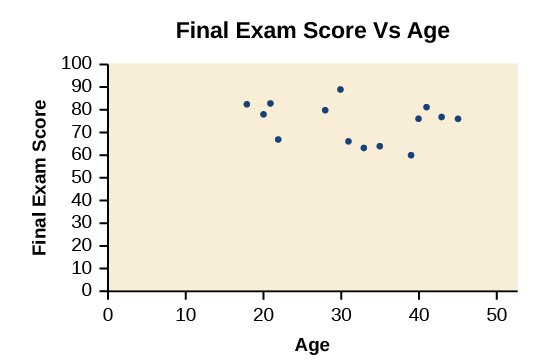
\includegraphics[scale=0.4]{finalExamVsAge.png}
\caption{\href{https://cnx.org/contents/mwjClAV_@8.12:6dX4RGdg@12/Fitting-Linear-Models-to-Data}{A scatterplot of age and final exam score variables}}
\end{figure}
$\answer[format=string]{No}$
\end{question}

\begin{question}
\begin{figure}
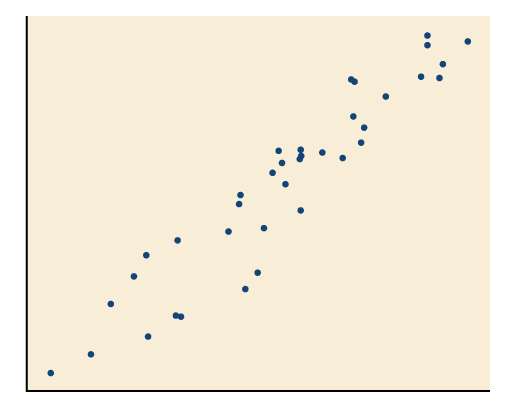
\includegraphics[scale=0.4]{positiveR.png}
\caption{\href{https://cnx.org/contents/mwjClAV_@8.12:6dX4RGdg@12/Fitting-Linear-Models-to-Data}{Scatterplot}}
\end{figure}
$\answer[format=string]{Yes}$
\end{question}

\begin{question}
\begin{figure}
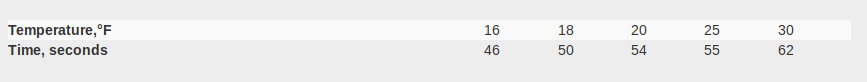
\includegraphics[scale=0.4]{temperature.png}
\caption{\href{https://cnx.org/contents/mwjClAV_@8.12:6dX4RGdg@12/Fitting-Linear-Models-to-Data}{Temperature over time (s).}}
\end{figure}
$\answer[format=string]{Yes}$
\end{question}

\begin{question}
\begin{figure}
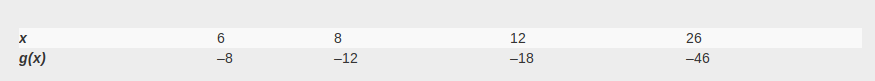
\includegraphics[scale=0.4]{tableFunction.png}
\caption{\href{https://cnx.org/contents/mwjClAV_@8.12:6dX4RGdg@12/Fitting-Linear-Models-to-Data}{Table of a function.}}
\end{figure}
$\answer[format=string]{No}$
\end{question}

\end{document}